\subsubsection*{Cost Category 22.01.08 Target Factory}

Prometheus scaling, and perhaps an exposition of the thinking of Miles et al, giving some examples of how the targets will be produced.\\

This cost category includes the cost of manufacturing and filling the hohlraum targets with DT fuel, assembling all the target components, LEH window cover manufacture, Cryostat costs, and  building costs, construction, maintenance and utilities and
personnel costs.


Cost category 22.01.08.01 process costs, are estimated from \cite{miles2008life} and comprise:

\begin{enumerate}
    \item Fabricate capsule ablator using a CVD diamond process. Diamon is selected as it meets the stringent geometric specifications for IFE capsules. The diamond is chemical vapour deposited (CVD) on silicone mandrels, polished, then the mandrel is etched out through a hole in the ablator. 
    \item Fill the capsule with DT mixture then seal. A hole is punched through the capsule wall and a droplet of DT is injected into the cavity, which is then sealed. For a full breakdown of the process tooling, see \cite{miles2008life}. 
    \item  Press two hohlraum halves per target.
    \item Produce two tents per target and attach to the hohlraum-halves. The tents are made of thin sheets of Formvar, a polyvinyl formal
polymer typically used for TEM sample preparation. They are described to be made by first spinning a Formvar-solvent solution onto a 12” silicon
wafer substrate which is dried in a conveyor oven then robotically scribed to delineate the tent membrane disks.
    \item Assemble filled capsule between two hohlraum-tent assemblies and
glue together.

    \item Apply LEH window covers to the gas-filled hohlraum. The LEH windows are currently made using 500 nm thick polyimide sheets. The
sheet can be laser cut then the discs robotically suctioned and placed on the
hohlraum LEH window which has had glue applied previously.
    \item Form the DT ice layer within the capsule.The DT inject process and the process to create the DT ice layer both require the equipment to be cooled to cryogenic temperatures. By considering the magnet cryogenic requirements at CERN, a cost can be found based on the volume required to be at cryogenic temperatures and the required cooling power.



\end{enumerate}

Cost category 22.01.08.02 factory costs includes e building costs, construction, maintenance and utilities and
personnel costs. Floorspace for production costs are estimated from the required tooling for each of the above process steps. construction costs were assumed to be \$250/sqrft Utilities were assumed to
be \$35/sqrft/yr [12]. Equipment maintenance was assumed to be 5\% of the
purchase price per year [12]. 

\begin{figure}
    \centering
    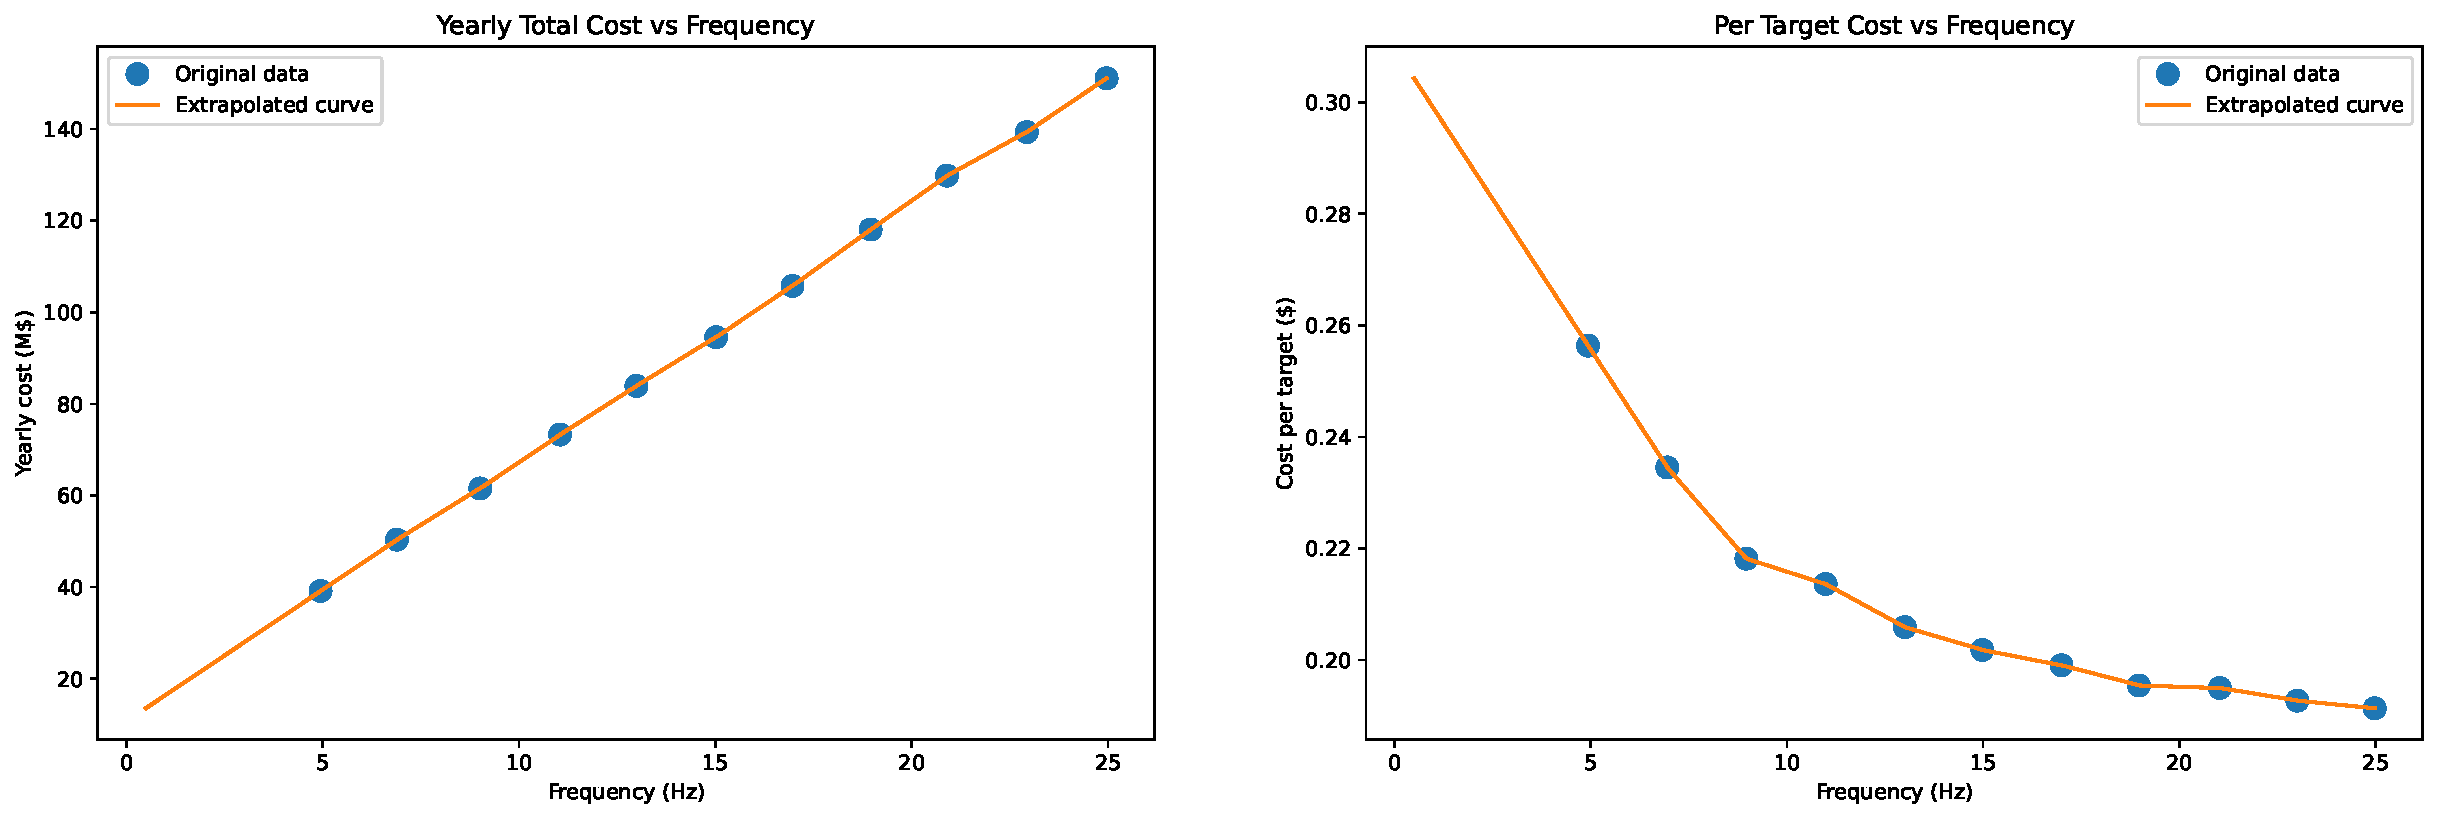
\includegraphics[width=0.9\linewidth]{Figures/targetPFR.pdf}
    \caption{The variation of individual (left) and total annual (right) target costs versus PFR (primary frequency response).}
    \label{fig:targetPFR}
\end{figure}



\begin{table}[h]
\centering
\resizebox{\linewidth}{!}{
\begin{tabular}{lcccccccc}
\hline
\textbf{Process machines} & \textbf{No. Machines} & \textbf{Floorspace (sqft)} & \textbf{WIP (parts)} & \textbf{TCC (M\$)} & \textbf{Annualized CC (\$/yr)} & \textbf{Consumables + electricity + maintenance} & \textbf{Personnel Costs (\$/yr)} & \textbf{Cost/target} \\
\hline
CVD diamond ablator & cvddiamondablatornomachines & cvddiamondablatorfloorspacesqrft & cvddiamondablatorwipparts & cvddiamondablatortccdollars & cvddiamondablatorannualizedccdollarsperyear & cvddiamondablatorconsumableselectricitymaint & cvddiamondablatorpersonnelcostsdollarsperyear & cvddiamondablatorcostpertarget \\
DT Fill & dtfillnomachines & dtfillfloorspacesqrft & dtfillwipparts & dtfilltccdollars & dtfillannualizedccdollarsperyear & dtfillconsumableselectricitymaint & dtfillpersonnelcostsdollarsperyear & dtfillcostpertarget \\
Hohlraum press & hohlraumpressnomachines & hohlraumpressfloorspacesqrft & hohlraumpresswipparts & hohlraumpresstccdollars & hohlraumpressannualizedccdollarsperyear & hohlraumpressconsumableselectricitymaint & hohlraumpresspersonnelcostsdollarsperyear & hohlraumpresscostpertarget \\
Tent assy & tentassynomachines & tentassyfloorspacesqrft & tentassywipparts & tentassytccdollars & tentassyannualizedccdollarsperyear & tentassyconsumableselectricitymaint & tentassypersonnelcostsdollarsperyear & tentassycostpertarget \\
Hohlraum-capsule assy & hohlraumcapsuleassynomachines & hohlraumcapsuleassyfloorspacesqrft & hohlraumcapsuleassywipparts & hohlraumcapsuleassytccdollars & hohlraumcapsuleassyannualizedccdollarsperyear & hohlraumcapsuleassyconsumableselectricitymaint & hohlraumcapsuleassypersonnelcostsdollarsperyear & hohlraumcapsuleassycostpertarget \\
LEH window attach & lehwindowattachnomachines & lehwindowattachfloorspacesqrft & lehwindowattachwipparts & lehwindowattachtccdollars & lehwindowattachannualizedccdollarsperyear & lehwindowattachconsumableselectricitymaint & lehwindowattachpersonnelcostsdollarsperyear & lehwindowattachcostpertarget \\
DT ice form & dticeformnomachines & dticeformfloorspacesqrft & dticeformwipparts & dticeformtccdollars & dticeformannualizedccdollarsperyear & dticeformconsumableselectricitymaint & dticeformpersonnelcostsdollarsperyear & dticeformcostpertarget \\
Recover and recycle & recoverandrecyclenomachines & recoverandrecyclefloorspacesqrft & recoverandrecyclewipparts & recoverandrecycletccdollars & recoverandrecycleannualizedccdollarsperyear & recoverandrecycleconsumableselectricitymaint & recoverandrecyclepersonnelcostsdollarsperyear & recoverandrecyclecostpertarget \\
Facility management costs & facilitymanagementcostsnomachines & facilitymanagementcostsfloorspacesqrft & facilitymanagementcostswipparts & facilitymanagementcoststccdollars & facilitymanagementcostsannualizedccdollarsperyear & facilitymanagementcostsconsumableselectricitymaint & facilitymanagementcostspersonnelcostsdollarsperyear & facilitymanagementcostscostpertarget \\
Total process & totalprocessnomachines & totalprocessfloorspacesqrft & totalprocesswipparts & totalprocesstccdollars & totalprocessannualizedccdollarsperyear & totalprocessconsumableselectricitymaint & totalprocesspersonnelcostsdollarsperyear & totalprocesscostpertarget \\
Add material & addmaterialnomachines & addmaterialfloorspacesqrft & addmaterialwipparts & addmaterialtccdollars & addmaterialannualizedccdollarsperyear & addmaterialconsumableselectricitymaint & addmaterialpersonnelcostsdollarsperyear & addmaterialcostpertarget \\
\hline
\end{tabular}}
\caption{Target factory costs and requirements.}
\label{tab:tfactory}
\end{table}




%he factory costs include building costs, construction, maintenance and utilities and personnel costs. The costs can be divided between factory management costs needed for a factory of any size and production costs based on the floorspace and numbers of machines needed for target production. Floorspace for factory management costs include office space for the fixed personnel (factory manager, assistant manager, administration, building maintenance and janitorial) lavatories and breakroom. Floorspace for production costs were estimated as the sum of the requirements for the factory equipment with an additional allowance for access to the machinery and the office space needed for variable personnel (process engineers, operators, and equipment maintenance personnel). There is assumed to
%be 1 process engineer for each 10 pieces of equipment. There are assumed to be 5 shifts needed for 24 hour operation so many personnel are multiplied by this factor. Process engineers are assumed to work a normal 5-day workweek. Construction costs were assumed to be \$250/sqft [12]. Utilities were assumed to be \$35/sqrft/yr [12]. Equipment maintenance was assumed to be 5% of the purchase price per year [12]. The annualized cost of capital was calculated by multiplying the total capital cost by a fixed charge rate of 7.7\%. The equipment replacement charge was calculated by dividing the equipment cost by the lifetime of the equipment. Equipment installation costs are included using a multiplier of 1.75 times the equipment cost.\\

 The total is thus C220108 M USD.
